% --------------------
% Packages
% -------------------
\documentclass[11pt,letter]{article}
\usepackage[top=1in, bottom=1in, left=1in, right=1in]{geometry}
%\usepackage[utf8x]{inputenc}
%\usepackage[T1]{fontenc}
\usepackage{times}
\usepackage[english]{babel} % Swedish translations
%
\usepackage[linkcolor=black,colorlinks=true,linkcolor=Blue,citecolor=Maroon, urlcolor=gray]{hyperref} 
\urlstyle{same}
\usepackage{enumitem} % Includes lists
\usepackage{amsmath}
\usepackage{amssymb}
\usepackage{mathrsfs}

\usepackage{graphicx}
\usepackage{float}
\usepackage{subcaption}

\captionsetup{
    width=0.9\textwidth, % width of caption is 90% of current textwidth
    labelfont=bf,        % the label, e.g. figure 12, is bold
    font={small,it},          % the whole caption text (label + content) is small
}
\usepackage{natbib}

\usepackage[usenames,dvipsnames]{color}
\usepackage{wrapfig} 
\usepackage[ruled,vlined]{algorithm2e}
\graphicspath{{figures/}}

\usepackage{tikz}
\newcommand{\ExternalLink}{%
    \tikz[x=1.2ex, y=1.2ex, baseline=-0.05ex]{% 
        \begin{scope}[x=1ex, y=1ex]
            \clip (-0.1,-0.1) 
                --++ (-0, 1.2) 
                --++ (0.6, 0) 
                --++ (0, -0.6) 
                --++ (0.6, 0) 
                --++ (0, -1);
            \path[draw, 
                line width = 0.5, 
                rounded corners=0.5] 
                (0,0) rectangle (1,1);
        \end{scope}
        \path[draw, line width = 0.5] (0.5, 0.5) 
            -- (1, 1);
        \path[draw, line width = 0.5] (0.6, 1) 
            -- (1, 1) -- (1, 0.6);
        }
    }



\SetKw{KwBy}{by}

\usepackage{mycommands}
\usepackage{shorthands}

% comments between authors
\newcommand{\tojeroen}[1]{\textbf{\green{*** Jeroen: #1 ***}}}
\newcommand{\torest}[1]{\textbf{\blue{*** Rest: #1 ***}}}

%-----------------------
% Set information such as title, author, etc.
%-----------------------
\title{RSE PROPOSAL}
\author{Jeroen Tromp}
\date\today

%-----------------------
% Change Header and Footer
%-----------------------
\usepackage{fancyhdr}
% \pagestyle{fancy}
% \fancyhf{}% Clear header/footer
% \fancyhead[L]{ORFEUS Software Development Grant Application}
% \fancyhead[R]{P. Makus}
% \fancyfoot[L]{}
% \fancyfoot[R]{\thepage}
% \renewcommand{\headrulewidth}{0.4pt}
% \renewcommand{\footrulewidth}{0.4pt}

%-----------------------
% No widows
%-----------------------
\widowpenalty10000
\clubpenalty10000

\begin{document}
%\thispagestyle{empty} % Suppress header and Footer on the first page
\noindent {\Large{\textbf{SPECFEM++: A Kokkos-based Spectral-Element Library for Wave Propagation Modeling and Imaging}}}
\vspace{-0.5em}\newline
\noindent\rule{\textwidth}{0.4pt}

\paragraph{Summary}

We propose to create a \software{Kokkos} version of the \SF\ software suite, which is used for simulating wave propagation and tomographic imaging. The resulting software will be hardware-agnostic and can be utilized beyond the exascale. Our team consists of one current RSE and two new RSEs, for which we are requesting 50\% university support (i.e., 1 FTE). This project presents an opportunity for the Princeton Research Computing community to gain expertise in programming models that focus on leveraging modern architectures. The RSEs graduating from this project will be well-equipped to support the increasing need for modernizing scientific codes across the university.

\section{SPECFEM}

The \SF\ software suite  (\href{https://specfem.org/}{specfem.org \ExternalLink})  is an open-source tool for simulating wave propagation and generating tomographic images. It can model 2D and 3D acoustic, (an)elastic, gravity, and ultrasound wave propagation while taking into account complexities such as attenuation, solid-body rotation, self-gravitation, bathymetry, topography, ellipticity, and fluid-solid and solid-solid interfaces. The software has adjoint-state capabilities and is used in various fields such as exploration seismology, earthquake seismology, helioseismology, planetary seismology, nondestructive testing, and medicine. Since its inception in 1999, over 230 publications have used the \software{SPECFEM} software suite, and the number of citations has exceeded 2500 per year (Figure~\ref{fig:citations}) with an h-index of 84 (\href{https://scholar.google.com/citations?user=bvjzHdUAAAAJ}{Google Scholar \ExternalLink}). The software has garnered over 600 stars on GitHub. \SF\ is written in \software{Fortran90} with support for \software{CUDA} and \software{OpenMP}.

\begin{figure}[!h]
    \centering
    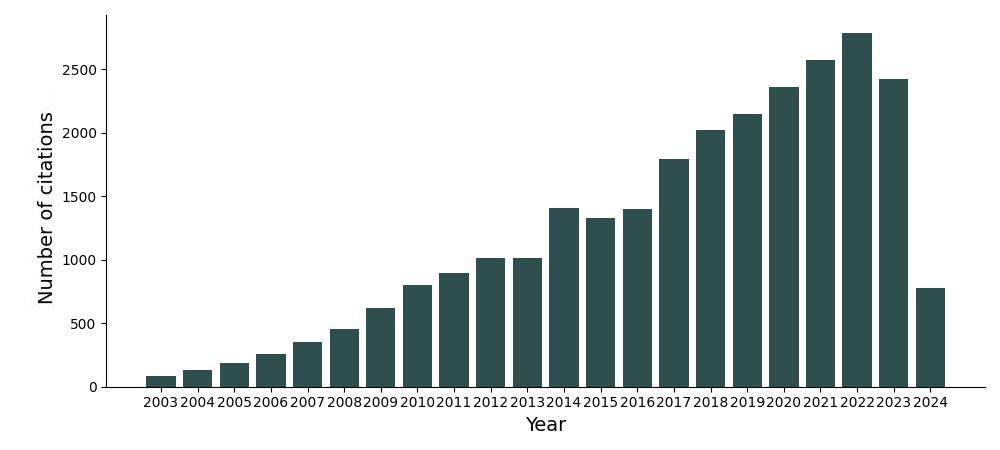
\includegraphics[width=0.85\textwidth, trim={.5cm .5cm 3.1cm .5cm}, clip]{figures/citations.png}
    \hspace{2.5em}
	\caption{We collected \SF\ publications on \href{https://scholar.google.com/citations?user=bvjzHdUAAAAJ}{Google Scholar} and counted their annual citations.}
	\label{fig:citations}
\end{figure}

\section{Kokkos}

\software{Kokkos} \citep{Trott2022} is a \software{C++} performance portability library that allows developers to write code without worrying about the underlying computing hardware. Thus, they can focus on underlying physics and algorithms. \software{Kokkos} uses \software{C++} templates to map different parallel execution patterns to target programming models like \software{CUDA}, \software{HIP}, \software{SYCL}, and \software{OpenMP}. Unlike other performance portability libraries such as \software{RAJA}, \software{OpenACC}, and \software{OpenMP}, \software{Kokkos} provides data management abstractions that maximize cache reuse, leading to better performance. \software{Kokkos} has been used to modernize several scientific codes, such as \software{LAAMPS}, \software{Trilinos}, and \software{PETSc}. At Princeton University, \software{Kokkos} has successfully helped to port a magnetohydrodynamics code developed by former PICSciE director Jim Stone to GPUs \citep{Stone2020}. The results show that Kokkos-enabled \software{Athena++} \citep{Grete2021} can achieve similar performance on CPUs while achieving a 30\% speedup compared to the native CUDA implementation on GPUs.

A major focus of the \software{Kokkos} team is fostering community engagement and increasing software usability based on user feedback. We have witnessed clear benefits in this regard, as the \software{Kokkos} team fast-tracked float SIMD vectorization support, a feature we requested, which should enable us to achieve better performance on CPUs beyond the current \software{SPECFEM} capabilities. Our team is in active contact with the \software{Kokkos} core developers, Christian Trott, Daniel Arndt, Damien Lebrun-Grandie, and Evan Harvey, through Slack and email. We presented our work at the \software{Kokkos} User Group Meeting in 2023.

\section{Research To Date}

Our goal is to develop a \SFPP\ library that provides an interface for developing spectral-element solvers in an architecture-independent manner. Currently, one RSE, Rohit Kakodkar, is the sole developer. He has laid the groundwork for integrating the core packages of \SF\ into a single interface using template metaprogramming. For simplicity, the focus has been on 2D wave propagation and imaging. The flexibility of dynamic code generation using templates at compile time has allowed him to develop a single interface while maintaining the performance of the original code base. However, a team of software engineers will be required to extend this proof-of-concept framework to simulate 3D wave propagation and perform tomographic inversions at high resolution and on a global scale.

\section{Proposed Research}

This proposal requests support for two additional research software engineers (RSE1 and RSE2), complementing RSE0 (Kakodkar). We request 50\% funding for RSE1 and RSE2 (1~FTE) for three years. The PI will provide the remaining 50\% of the funding. The project is divided into three stages as follows.

\subsection{Stage 1: Development of forward-adjoint solvers (September 2024--August 2025)}

\begin{figure}[!ht]
    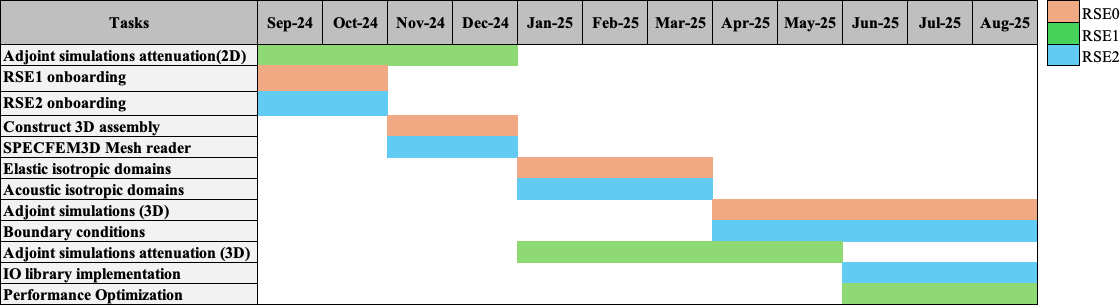
\includegraphics[width=0.975\textwidth]{figures/stage1.png}
    \caption{GANTT chart of the tasks for the three RSEs planned for the first year.}
    \label{fig:stage1}
\end{figure}

The project's first stage (Figure~\ref{fig:stage1}) will focus on developing a forward-adjoint solver for 2D and 3D seismic wave propagation. On completion, the solver should provide 75--80\% of the functionality primarily used by the \SF\ community, i.e., functionally required to compute tomographic models. This will enable us to onboard the \SF\ community (users and developers) to the \SFPP\ framework and gather feedback on the usability and performance of the framework. The GANTT chart in Figure~\ref{fig:stage1} provides a high-level overview of this stage's planned tasks and the distribution of work between the RSEs. The goal is to familiarize the two new RSEs with the \SFPP\ framework and have them independently contribute to developing the 3D solver.

\subsection{Stage 2: Support for global tomography (September 2025--April 2026)}


\begin{figure}[!h] 
    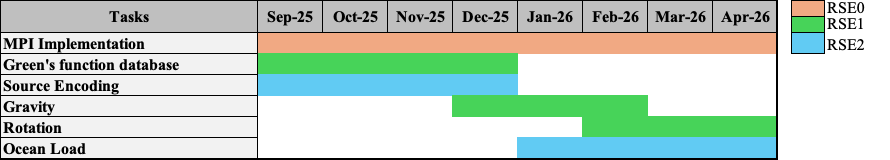
\includegraphics[width=0.8\textwidth]{figures/stage2.png}
        \caption{GANTT chart of the tasks for the three RSEs planned for the second year.}
    \label{fig:stage2}
\end{figure}


The second stage of the project (Figure~\ref{fig:stage2}) will provide support for simulating seismic wave propagation on a global scale. Such simulations require additional features to incorporate the effects of Earth's curvature, rotation, gravity, and ocean load. Additionally, computing global-scale tomographic models will require extending the framework to run across multiple nodes using \software{MPI}. While the current \SF\ packages provide \software{MPI} support through direct \software{MPI} library calls, we would also like to explore using \software{PETSc} (i.e., \software{DMplex} vectors) to manage the distribution/communication of the mesh across nodes using \software{MPI}. This approach has proven successful in spectral-element libraries like \software{libCEED} \citep{Abdelfattah2021}. Lastly, combining recent developments from our group, such as source encoding \citep{Tromp2019, Bachmann2020, Cui2023} and Green’s function databases \citep{Sawade2024}, with the \SFPP\ framework will enable us to compute global-scale tomographic models efficiently. On completion, the solver should provide 90--95\% of the functionality of the original \SF\ code base.

\subsection{Stage 3: Extension beyond current \software{SPECFEM} capabilities (May 2026--May 2027)}

\begin{figure}[!hb]
    \centering
    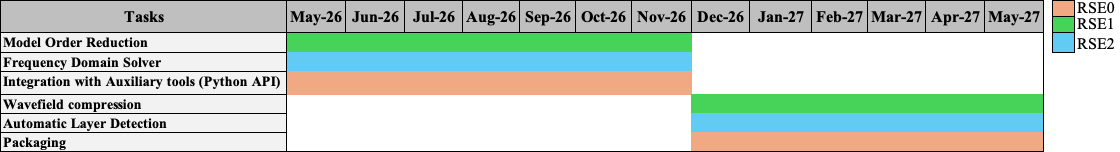
\includegraphics[width=\textwidth]{figures/stage3.png}
    \caption{GANTT chart of the tasks for the three RSEs planned for the third year.}
    \label{fig:stage3}
\end{figure}

The third stage of the project (Figure~\ref{fig:stage3}) has two main goals.
First, we will polish the product further based on community and user feedback and improve user-friendliness so that students or less seismology-oriented research groups can adopt the software. This step involves building an active community, making the interface consistent and intuitive, requiring as few human operations as possible, and adding step-by-step guides to configure \SF\ easily. We have been collaborating with people from geodynamics, mineral physics, and geochemistry, and they all have a certain degree of need for seismic wave simulation and tomography. Just making \SF\ more user-friendly can significantly increase its potential audience. 
Second, extend the capability of \SF\ to facilitate the latest scientific development, including but not limited to model order reduction \citep{Hawkins2023}, wavefield compression \citep{Boehm2016}, frequency domain solver \citep{Gharti2023}, and automatic mesh layer detection. These developments require more effort than standard \SF\ features but will have major impacts when successfully implemented.




\newpage

\bibliographystyle{abbrv}
\bibliography{bibliography}


\end{document}
